\documentclass{standalone}
\usepackage{tikz}
\usetikzlibrary{patterns, positioning}
\usepackage[sfdefault]{ClearSans} %% option 'sfdefault' activates Clear Sans as the default text font
\usepackage[T1]{fontenc}

\begin{document}
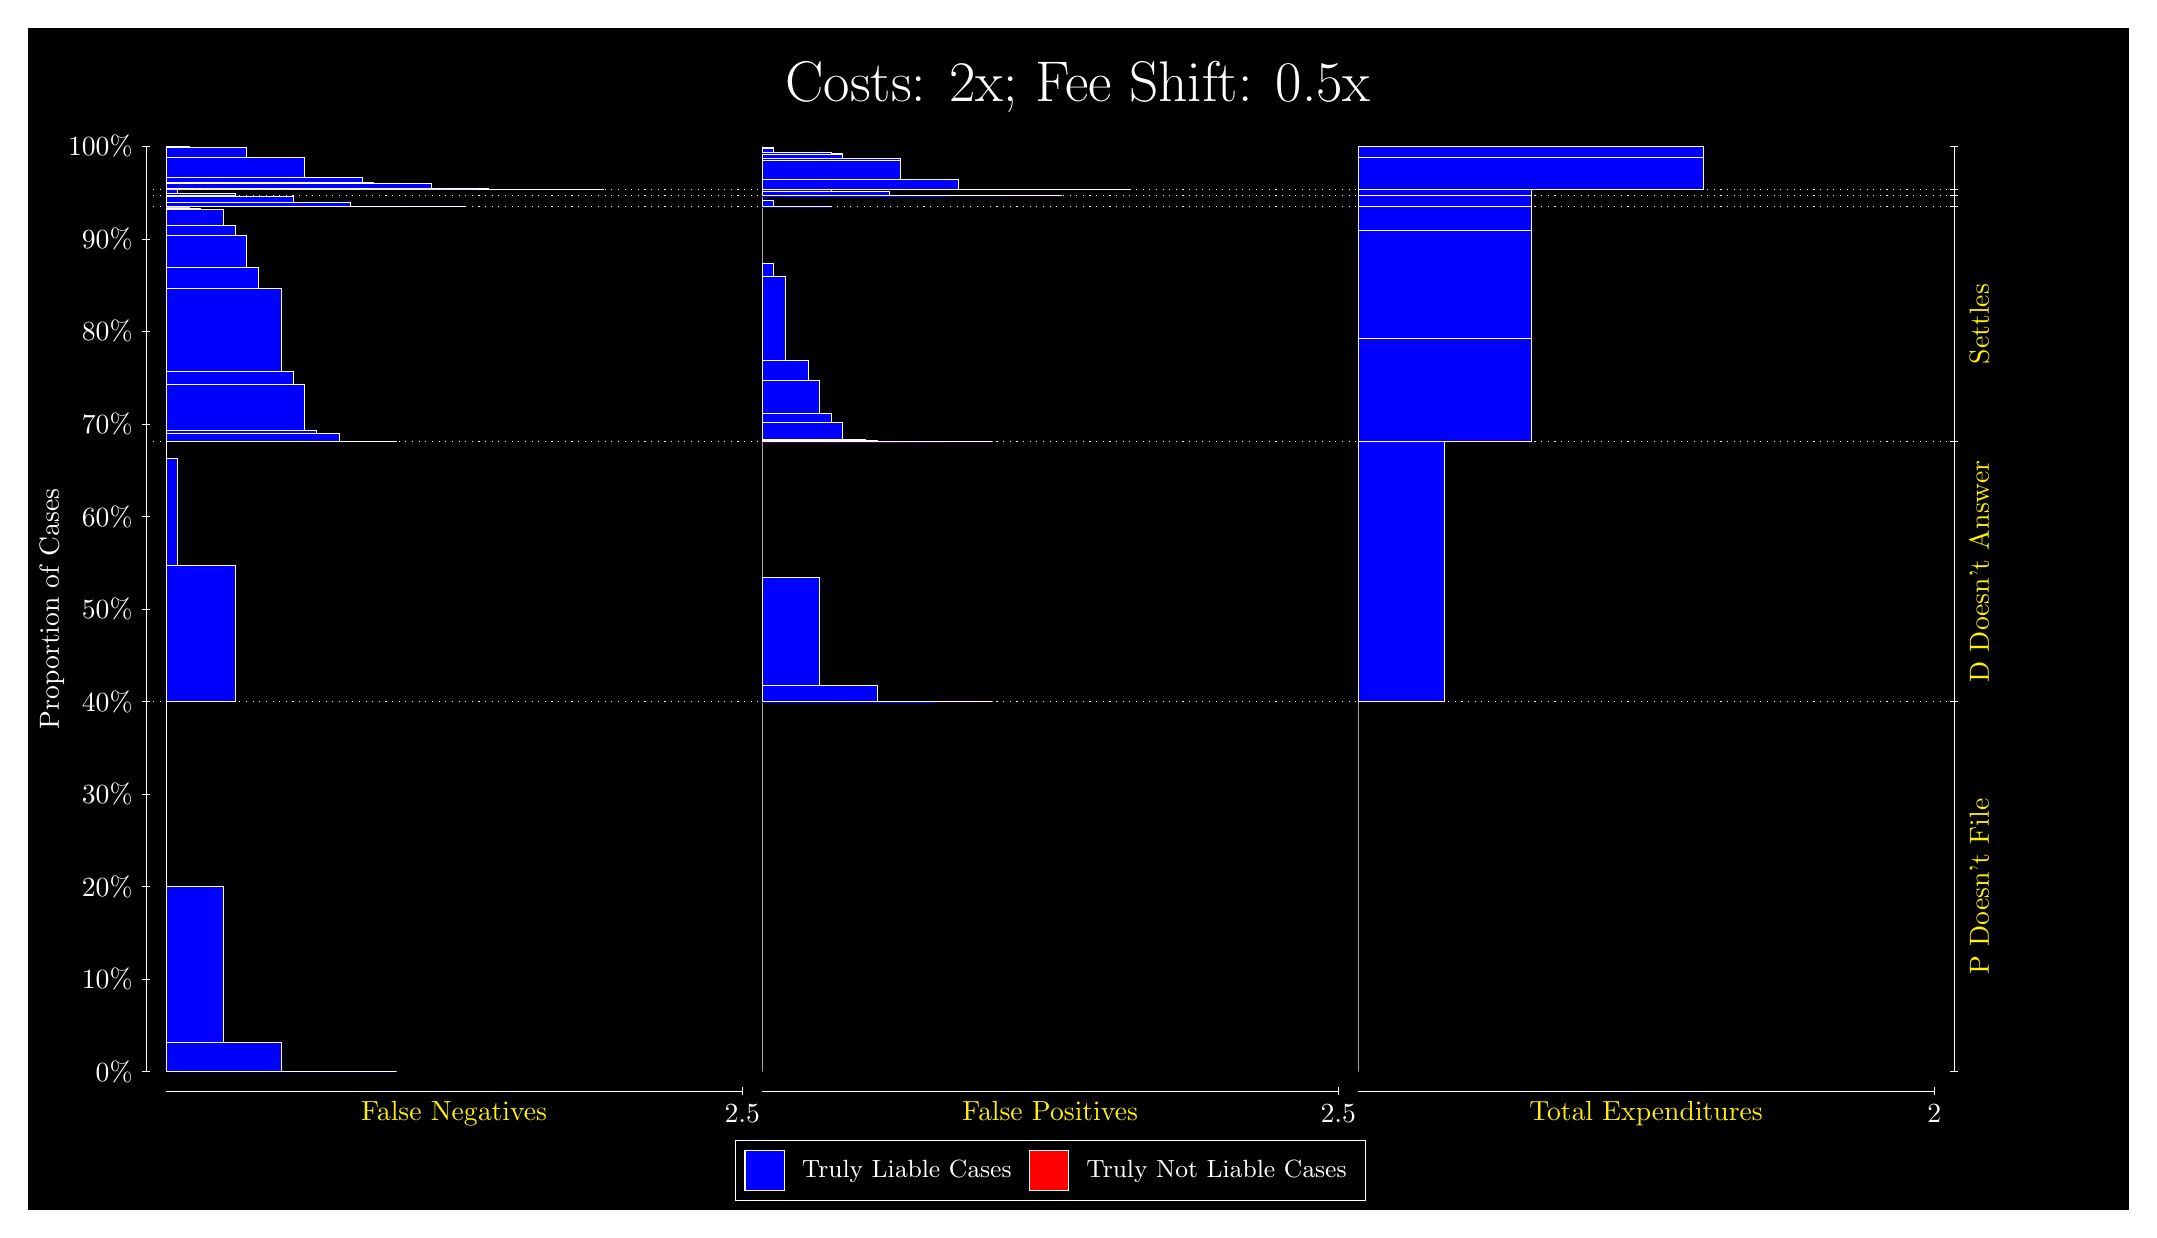
\begin{tikzpicture}
\draw[fill=black] (0,0) rectangle (26.667,15);
\draw[text=white] (0,13.5) rectangle (26.667,15) node[midway] {\huge Costs: 2x; Fee Shift: 0.5x};
\draw[white, very thin] (1.5,1.75) -- (1.5,13.5);
\node[rotate=90, text=white, anchor=center] at (0.3, 7.625) {Proportion of Cases};
\draw[white, very thin] (1.45,1.75) -- (1.55,1.75);
\node[text=white, anchor=east] at (1.45, 1.75) {0\%};
\draw[white, very thin] (1.45,2.925) -- (1.55,2.925);
\node[text=white, anchor=east] at (1.45, 2.925) {10\%};
\draw[white, very thin] (1.45,4.1) -- (1.55,4.1);
\node[text=white, anchor=east] at (1.45, 4.1) {20\%};
\draw[white, very thin] (1.45,5.275) -- (1.55,5.275);
\node[text=white, anchor=east] at (1.45, 5.275) {30\%};
\draw[white, very thin] (1.45,6.45) -- (1.55,6.45);
\node[text=white, anchor=east] at (1.45, 6.45) {40\%};
\draw[white, very thin] (1.45,7.625) -- (1.55,7.625);
\node[text=white, anchor=east] at (1.45, 7.625) {50\%};
\draw[white, very thin] (1.45,8.8) -- (1.55,8.8);
\node[text=white, anchor=east] at (1.45, 8.8) {60\%};
\draw[white, very thin] (1.45,9.975) -- (1.55,9.975);
\node[text=white, anchor=east] at (1.45, 9.975) {70\%};
\draw[white, very thin] (1.45,11.15) -- (1.55,11.15);
\node[text=white, anchor=east] at (1.45, 11.15) {80\%};
\draw[white, very thin] (1.45,12.325) -- (1.55,12.325);
\node[text=white, anchor=east] at (1.45, 12.325) {90\%};
\draw[white, very thin] (1.45,13.5) -- (1.55,13.5);
\node[text=white, anchor=east] at (1.45, 13.5) {100\%};

\draw[white, very thin] (24.457,1.75) -- (24.457,13.5);
\draw[white, very thin] (24.407,1.75) -- (24.507,1.75);
\node[anchor=west] at (24.407, 1.75) {};
\draw[white, very thin] (24.407,6.4489) -- (24.507,6.4489);
\node[anchor=west] at (24.407, 6.4489) {};
\draw[white, very thin] (24.407,9.7509) -- (24.507,9.7509);
\node[anchor=west] at (24.407, 9.7509) {};
\draw[white, very thin] (24.407,12.733) -- (24.507,12.733);
\node[anchor=west] at (24.407, 12.733) {};
\draw[white, very thin] (24.407,12.873) -- (24.507,12.873);
\node[anchor=west] at (24.407, 12.873) {};
\draw[white, very thin] (24.407,12.953) -- (24.507,12.953);
\node[anchor=west] at (24.407, 12.953) {};
\draw[white, very thin] (24.407,13.5) -- (24.507,13.5);
\node[anchor=west] at (24.407, 13.5) {};

\draw[white, very thin, fill=blue] (1.75,1.75) rectangle (4.6775,1.75);
\draw[white, very thin, fill=blue] (1.75,1.75) rectangle (3.9457,1.7532);
\draw[white, very thin, fill=blue] (1.75,1.7532) rectangle (3.2138,2.126);
\draw[white, very thin, fill=blue] (1.75,2.126) rectangle (2.4819,4.1027);
\draw[white, very thin, fill=red] (1.75,4.1027) rectangle (1.75,4.1027);
\draw[white, very thin, fill=blue] (1.75,4.1027) rectangle (1.75,6.4489);
\draw[white, very thin, fill=blue] (1.75,6.4489) rectangle (2.6283,8.1761);
\draw[white, very thin, fill=blue] (1.75,8.1761) rectangle (1.8964,9.5382);
\draw[white, very thin, fill=red] (1.75,9.5382) rectangle (1.75,9.5382);
\draw[white, very thin, fill=blue] (1.75,9.5382) rectangle (1.75,9.7509);
\draw[white, very thin, fill=blue] (1.75,9.7509) rectangle (4.6775,9.7514);
\draw[white, very thin, fill=blue] (1.75,9.7514) rectangle (4.3848,9.7514);
\draw[white, very thin, fill=blue] (1.75,9.7514) rectangle (4.092,9.7559);
\draw[white, very thin, fill=blue] (1.75,9.7559) rectangle (3.9457,9.86);
\draw[white, very thin, fill=blue] (1.75,9.86) rectangle (3.6529,9.8878);
\draw[white, very thin, fill=blue] (1.75,9.8878) rectangle (3.5065,10.473);
\draw[white, very thin, fill=blue] (1.75,10.473) rectangle (3.3602,10.637);
\draw[white, very thin, fill=blue] (1.75,10.637) rectangle (3.2138,11.703);
\draw[white, very thin, fill=blue] (1.75,11.703) rectangle (2.921,11.958);
\draw[white, very thin, fill=blue] (1.75,11.958) rectangle (2.7746,12.374);
\draw[white, very thin, fill=blue] (1.75,12.374) rectangle (2.6283,12.494);
\draw[white, very thin, fill=blue] (1.75,12.494) rectangle (2.4819,12.704);
\draw[white, very thin, fill=blue] (1.75,12.704) rectangle (2.1891,12.717);
\draw[white, very thin, fill=blue] (1.75,12.717) rectangle (2.0428,12.732);
\draw[white, very thin, fill=blue] (1.75,12.732) rectangle (1.8964,12.733);
\draw[white, very thin, fill=red] (1.75,12.733) rectangle (1.75,12.733);
\draw[white, very thin, fill=blue] (1.75,12.733) rectangle (1.75,12.733);
\draw[white, very thin, fill=blue] (1.75,12.733) rectangle (5.5558,12.733);
\draw[white, very thin, fill=blue] (1.75,12.733) rectangle (4.8239,12.733);
\draw[white, very thin, fill=blue] (1.75,12.733) rectangle (4.092,12.786);
\draw[white, very thin, fill=blue] (1.75,12.786) rectangle (3.3602,12.871);
\draw[white, very thin, fill=blue] (1.75,12.871) rectangle (2.6283,12.873);
\draw[white, very thin, fill=red] (1.75,12.873) rectangle (1.75,12.873);
\draw[white, very thin, fill=blue] (1.75,12.873) rectangle (2.6283,12.901);
\draw[white, very thin, fill=blue] (1.75,12.901) rectangle (1.8964,12.951);
\draw[white, very thin, fill=red] (1.75,12.951) rectangle (1.75,12.951);
\draw[white, very thin, fill=blue] (1.75,12.951) rectangle (1.75,12.953);
\draw[white, very thin, fill=blue] (1.75,12.953) rectangle (7.3123,12.953);
\draw[white, very thin, fill=blue] (1.75,12.953) rectangle (6.5805,12.953);
\draw[white, very thin, fill=blue] (1.75,12.953) rectangle (5.8486,12.963);
\draw[white, very thin, fill=blue] (1.75,12.963) rectangle (5.7022,12.963);
\draw[white, very thin, fill=blue] (1.75,12.963) rectangle (5.1167,13.032);
\draw[white, very thin, fill=blue] (1.75,13.032) rectangle (4.9703,13.032);
\draw[white, very thin, fill=blue] (1.75,13.032) rectangle (4.3848,13.044);
\draw[white, very thin, fill=blue] (1.75,13.044) rectangle (4.2384,13.103);
\draw[white, very thin, fill=blue] (1.75,13.103) rectangle (3.6529,13.103);
\draw[white, very thin, fill=blue] (1.75,13.103) rectangle (3.5065,13.366);
\draw[white, very thin, fill=blue] (1.75,13.366) rectangle (2.921,13.366);
\draw[white, very thin, fill=blue] (1.75,13.366) rectangle (2.7746,13.493);
\draw[white, very thin, fill=blue] (1.75,13.493) rectangle (2.0428,13.5);
\draw[white, very thin, fill=red] (1.75,13.5) rectangle (1.75,13.5);
\draw[white, very thin, fill=blue] (1.75,13.5) rectangle (1.75,13.5);
\draw[white, very thin, fill=red] (9.3189,1.75) rectangle (9.3189,1.75);
\draw[white, very thin, fill=blue] (9.3189,1.75) rectangle (9.3189,6.4489);
\draw[white, very thin, fill=red] (9.3189,6.4489) rectangle (12.246,6.4489);
\draw[white, very thin, fill=blue] (9.3189,6.4489) rectangle (12.246,6.4489);
\draw[white, very thin, fill=blue] (9.3189,6.4489) rectangle (11.515,6.4493);
\draw[white, very thin, fill=blue] (9.3189,6.4493) rectangle (10.783,6.6616);
\draw[white, very thin, fill=blue] (9.3189,6.6616) rectangle (10.051,8.0237);
\draw[white, very thin, fill=blue] (9.3189,8.0237) rectangle (9.3189,9.7509);
\draw[white, very thin, fill=red] (9.3189,9.7509) rectangle (12.246,9.7509);
\draw[white, very thin, fill=blue] (9.3189,9.7509) rectangle (12.246,9.7509);
\draw[white, very thin, fill=red] (9.3189,9.7509) rectangle (11.661,9.7509);
\draw[white, very thin, fill=blue] (9.3189,9.7509) rectangle (11.661,9.7509);
\draw[white, very thin, fill=blue] (9.3189,9.7509) rectangle (11.515,9.7509);
\draw[white, very thin, fill=red] (9.3189,9.7509) rectangle (11.368,9.7509);
\draw[white, very thin, fill=blue] (9.3189,9.7509) rectangle (11.368,9.7509);
\draw[white, very thin, fill=red] (9.3189,9.7509) rectangle (11.075,9.7509);
\draw[white, very thin, fill=blue] (9.3189,9.7509) rectangle (11.075,9.7513);
\draw[white, very thin, fill=blue] (9.3189,9.7513) rectangle (10.929,9.7523);
\draw[white, very thin, fill=blue] (9.3189,9.7523) rectangle (10.783,9.7671);
\draw[white, very thin, fill=blue] (9.3189,9.7671) rectangle (10.636,9.7799);
\draw[white, very thin, fill=blue] (9.3189,9.7799) rectangle (10.344,9.99);
\draw[white, very thin, fill=blue] (9.3189,9.99) rectangle (10.197,10.11);
\draw[white, very thin, fill=blue] (9.3189,10.11) rectangle (10.051,10.526);
\draw[white, very thin, fill=blue] (9.3189,10.526) rectangle (9.9044,10.781);
\draw[white, very thin, fill=blue] (9.3189,10.781) rectangle (9.6116,11.847);
\draw[white, very thin, fill=blue] (9.3189,11.847) rectangle (9.4652,12.01);
\draw[white, very thin, fill=blue] (9.3189,12.01) rectangle (9.3189,12.733);
\draw[white, very thin, fill=red] (9.3189,12.733) rectangle (10.197,12.733);
\draw[white, very thin, fill=blue] (9.3189,12.733) rectangle (10.197,12.735);
\draw[white, very thin, fill=blue] (9.3189,12.735) rectangle (9.4652,12.819);
\draw[white, very thin, fill=blue] (9.3189,12.819) rectangle (9.3189,12.873);
\draw[white, very thin, fill=red] (9.3189,12.873) rectangle (13.125,12.873);
\draw[white, very thin, fill=blue] (9.3189,12.873) rectangle (13.125,12.873);
\draw[white, very thin, fill=blue] (9.3189,12.873) rectangle (12.393,12.873);
\draw[white, very thin, fill=blue] (9.3189,12.873) rectangle (11.661,12.874);
\draw[white, very thin, fill=blue] (9.3189,12.874) rectangle (10.929,12.924);
\draw[white, very thin, fill=blue] (9.3189,12.924) rectangle (10.197,12.953);
\draw[white, very thin, fill=red] (9.3189,12.953) rectangle (14.003,12.953);
\draw[white, very thin, fill=blue] (9.3189,12.953) rectangle (14.003,12.953);
\draw[white, very thin, fill=red] (9.3189,12.953) rectangle (13.271,12.953);
\draw[white, very thin, fill=blue] (9.3189,12.953) rectangle (13.271,12.953);
\draw[white, very thin, fill=red] (9.3189,12.953) rectangle (12.539,12.953);
\draw[white, very thin, fill=blue] (9.3189,12.953) rectangle (12.539,12.96);
\draw[white, very thin, fill=blue] (9.3189,12.96) rectangle (11.807,13.086);
\draw[white, very thin, fill=red] (9.3189,13.086) rectangle (11.807,13.086);
\draw[white, very thin, fill=blue] (9.3189,13.086) rectangle (11.807,13.086);
\draw[white, very thin, fill=red] (9.3189,13.086) rectangle (11.661,13.086);
\draw[white, very thin, fill=blue] (9.3189,13.086) rectangle (11.661,13.086);
\draw[white, very thin, fill=blue] (9.3189,13.086) rectangle (11.075,13.318);
\draw[white, very thin, fill=blue] (9.3189,13.318) rectangle (11.075,13.35);
\draw[white, very thin, fill=red] (9.3189,13.35) rectangle (10.929,13.35);
\draw[white, very thin, fill=blue] (9.3189,13.35) rectangle (10.929,13.35);
\draw[white, very thin, fill=blue] (9.3189,13.35) rectangle (10.344,13.395);
\draw[white, very thin, fill=blue] (9.3189,13.395) rectangle (10.344,13.409);
\draw[white, very thin, fill=blue] (9.3189,13.409) rectangle (10.197,13.42);
\draw[white, very thin, fill=red] (9.3189,13.42) rectangle (10.197,13.42);
\draw[white, very thin, fill=blue] (9.3189,13.42) rectangle (10.197,13.421);
\draw[white, very thin, fill=blue] (9.3189,13.421) rectangle (9.6116,13.421);
\draw[white, very thin, fill=blue] (9.3189,13.421) rectangle (9.6116,13.421);
\draw[white, very thin, fill=blue] (9.3189,13.421) rectangle (9.4652,13.474);
\draw[white, very thin, fill=blue] (9.3189,13.474) rectangle (9.4652,13.489);
\draw[white, very thin, fill=blue] (9.3189,13.489) rectangle (9.3189,13.5);
\draw[white, very thin, fill=red] (16.888,1.75) rectangle (16.888,1.75);
\draw[white, very thin, fill=blue] (16.888,1.75) rectangle (16.888,6.4489);
\draw[white, very thin, fill=red] (16.888,6.4489) rectangle (17.986,6.4489);
\draw[white, very thin, fill=blue] (16.888,6.4489) rectangle (17.986,9.7509);
\draw[white, very thin, fill=red] (16.888,9.7509) rectangle (19.083,9.7509);
\draw[white, very thin, fill=blue] (16.888,9.7509) rectangle (19.083,11.056);
\draw[white, very thin, fill=red] (16.888,11.056) rectangle (19.083,11.056);
\draw[white, very thin, fill=blue] (16.888,11.056) rectangle (19.083,12.437);
\draw[white, very thin, fill=red] (16.888,12.437) rectangle (19.083,12.437);
\draw[white, very thin, fill=blue] (16.888,12.437) rectangle (19.083,12.733);
\draw[white, very thin, fill=red] (16.888,12.733) rectangle (19.083,12.733);
\draw[white, very thin, fill=blue] (16.888,12.733) rectangle (19.083,12.873);
\draw[white, very thin, fill=red] (16.888,12.873) rectangle (19.083,12.873);
\draw[white, very thin, fill=blue] (16.888,12.873) rectangle (19.083,12.953);
\draw[white, very thin, fill=red] (16.888,12.953) rectangle (21.279,12.953);
\draw[white, very thin, fill=blue] (16.888,12.953) rectangle (21.279,13.363);
\draw[white, very thin, fill=red] (16.888,13.363) rectangle (21.279,13.363);
\draw[white, very thin, fill=blue] (16.888,13.363) rectangle (21.279,13.5);
\draw[white, dotted] (1.5,6.4489) -- (24.457,6.4489);
\draw[white, dotted] (1.5,9.7509) -- (24.457,9.7509);
\draw[white, dotted] (1.5,12.733) -- (24.457,12.733);
\draw[white, dotted] (1.5,12.873) -- (24.457,12.873);
\draw[white, dotted] (1.5,12.953) -- (24.457,12.953);
\draw[white, very thin] (1.75,1.5) -- (9.0689,1.5);
\node[text=yellow, anchor=north] at (5.4094, 1.5) {False Negatives};
\draw[white, very thin] (9.0689,1.45) -- (9.0689,1.55);
\node[text=white, anchor=north] at (9.0689, 1.45) {2.5};

\draw[white, very thin] (9.3189,1.5) -- (16.638,1.5);
\node[text=yellow, anchor=north] at (12.978, 1.5) {False Positives};
\draw[white, very thin] (16.638,1.45) -- (16.638,1.55);
\node[text=white, anchor=north] at (16.638, 1.45) {2.5};

\draw[white, very thin] (16.888,1.5) -- (24.207,1.5);
\node[text=yellow, anchor=north] at (20.547, 1.5) {Total Expenditures};
\draw[white, very thin] (24.207,1.45) -- (24.207,1.55);
\node[text=white, anchor=north] at (24.207, 1.45) {2};

\node[text=yellow, centered, rotate=90] at (24.777, 4.0995) {P Doesn't File};
\node[text=yellow, centered, rotate=90] at (24.777, 8.0999) {D Doesn't Answer};
\node[text=yellow, centered, rotate=90] at (24.777, 11.242) {Settles};




\draw (12.978300999999998,1.5) node[draw=none] (baseCoordinate) {};
\begin{scope}[align=center]
        \matrix[scale=0.5, draw=white, below=0.5cm of baseCoordinate, nodes={draw}, column sep=0.1cm]{
            \node[rectangle, draw, minimum width=0.5cm, minimum height=0.5cm, fill=blue] {}; &
            \node[draw=none, font=\small, text=white] (B) {Truly Liable Cases}; &
            \node[rectangle, draw, minimum width=0.5cm, minimum height=0.5cm, fill=red] {}; &
            \node[draw=none, font=\small, text=white] (B) {Truly Not Liable Cases}; \\
            };
\end{scope}

\end{tikzpicture}
\end{document}